\documentclass[conference]{IEEEtran}
\IEEEoverridecommandlockouts
\usepackage[utf8]{inputenc}
\usepackage[T1]{fontenc}
\usepackage{amsmath,amssymb}
\usepackage{graphicx}
\usepackage{booktabs}
\usepackage{xcolor}
\usepackage{url}
\usepackage[hidelinks]{hyperref}
\usepackage{cite}
\graphicspath{{figures/}}

\newcommand{\deltaMain}{$-$0.013}
\newcommand{\ciMain}{[$-$0.027, +0.002]}
\newcommand{\resBetter}{7 of 24}
\newcommand{\eegBetter}{17}
\newcommand{\resMainSubj}{0.761}
\newcommand{\eegMainSubj}{0.774}
\newcommand{\hypVerdict}{not supported}
\newcommand{\mainVerdict}{the interval includes zero, so the CNN on scalograms is not better than EEGNet on the raw signal; the two are statistically indistinguishable.}
\newcommand{\deltaInitial}{$-$0.005}
\newcommand{\deltaOldLr}{$-$0.024}
\newcommand{\ciOldLr}{[$-$0.037, $-$0.009]}
\newcommand{\oldLrSubj}{0.750}
\newcommand{\oldLrBetter}{5 of 24}
\newcommand{\deltaLrGain}{+0.011}
\newcommand{\ciLrGain}{[+0.005, +0.017]}
\newcommand{\lrGainBetter}{18 of 24}
\newcommand{\deltaCuda}{$-$0.007}
\newcommand{\ciCuda}{[$-$0.023, +0.009]}
\newcommand{\deltaCudaMps}{+0.006}
\newcommand{\ciCudaMps}{[$-$0.002, +0.013]}
\newcommand{\deltaCudaPair}{+0.000}
\newcommand{\ciCudaPair}{[$-$0.015, +0.017]}
\newcommand{\deltaStftCuda}{+0.006}
\newcommand{\ciStftCuda}{[$-$0.000, +0.012]}
\newcommand{\deltaScratch}{+0.015}
\newcommand{\ciScratch}{[+0.004, +0.025]}
\newcommand{\scratchSubj}{0.735}
\newcommand{\deltaStft}{+0.007}
\newcommand{\ciStft}{[$-$0.005, +0.019]}
\newcommand{\stftSubj}{0.755}
\newcommand{\deltaStftOld}{$-$0.001}
\newcommand{\ciStftOld}{[$-$0.010, +0.007]}
\newcommand{\stftVerdict}{indistinguishably}
\newcommand{\stftSentence}{the interval includes zero, so the choice of time--frequency transform does not measurably matter here.}
\newcommand{\stftShort}{makes no measurable difference}
\newcommand{\worstRange}{0.65 to 0.89 for EEGNet}
\newcommand{\worstSubjects}{22 (0.65, 51\% slow), 9 (0.69, 34\% slow), 31 (0.71, 21\% slow), 6 (0.71, 20\% slow)}
\newcommand{\condText}{0.791 (motion) vs.\ 0.782 (motionless) for EEGNet and 0.759 vs.\ 0.760 for ResNet18; a descriptive, not pre-registered, contrast.}
\newcommand{\agreePct}{86.2\%}
\newcommand{\disagree}{EEGNet 58.3\% vs.\ ResNet18 41.7\%}
\newcommand{\bothWrongSlow}{32.2\%}


\begin{document}

\title{Images or Raw Signal? Decoding a Subject-Relative\\ Response State from Pre-Event EEG on Unseen Subjects}

\author{\IEEEauthorblockN{Juan Pablo Acevedo Robles and Alberto Martinez Hernandez}
\IEEEauthorblockA{Team 8 -- Deep Learning, Final Project}}

\maketitle

\begin{abstract}
Inferring subjective states from EEG is hard because the signal varies strongly between people, so a model must be judged on subjects it has never seen. We isolate one design choice that recurs in our two doctoral projects (trust in autonomous systems and pain quantification): whether converting EEG into time--frequency images for an ImageNet-pretrained CNN generalizes better than a compact network on the raw signal. On a public sustained-attention driving dataset (26 subjects, 18{,}087 windows), we predict from the 3\,s of EEG (Fz, Pz, Oz) before a lane deviation whether the driver's response will be fast or slow relative to their own session. With 5-fold subject-wise cross-validation, 3 seeds, a matched tuning budget, and a pre-registered decision rule, a ResNet18 on wavelet scalograms reaches \resMainSubj{} per-subject balanced accuracy versus \eegMainSubj{} for EEGNet on the raw signal ($\Delta=\deltaMain$, 95\% subject-bootstrap CI \ciMain). The hypothesis that images help is not supported. Ablations show that ImageNet pretraining helps the CNN (\deltaScratch) and that wavelets and short-time Fourier spectrograms perform \stftVerdict{}. A channel and band diagnostic indicates that a large share of the information is in frontal delta activity, which may be partly ocular, and we report this as the main limitation.
\end{abstract}

\section{Introduction and thesis context}
Both authors infer subjective states from EEG. Juan Pablo studies real-time measurement of trust in autonomous systems from physiological signals, with autonomous driving as the testbed. Alberto studies the quantification and standardization of pain from EEG: the clinical standard is still self-report (e.g., a 0--10 numerical rating scale), which is subjective, requires the person to communicate, and is not comparable across people~\cite{davis2017}. An EEG marker could give a more objective measure~\cite{ploner2018}, but pain-related cortical activity varies strongly between individuals, so a useful model must work on people it has not seen.

The two theses share a methodological question: \emph{which EEG representation generalizes best to new people when the target is a state defined relative to each person?} Both of our own datasets are still being collected (target: at least 40 subjects each) and will not be ready for this project. We therefore use a complete public dataset~\cite{cao2019} as a testbed to build and validate the pipeline. The link to the theses is indirect: this dataset measures neither trust nor pain. Its label, a reaction time made relative to each session, plays the role that a per-person-normalized trust or pain rating will play in our own data.

\textbf{Sub-objective.} Predict, from the EEG before an event, whether a driver's response will be fast or slow, and measure whether a time--frequency image representation improves generalization to unseen subjects compared with the raw signal.

\section{Problem formulation and hypothesis}
\textbf{Task.} Supervised, discriminative binary classification evaluated across subjects.

\textbf{Input.} A 3\,s window of EEG ending at lane-deviation onset (markers 251/252), channels Fz, Pz, Oz, band-pass 1--50\,Hz and resampled to 250\,Hz: $x\in\mathbb{R}^{3\times750}$. The CNN instead receives a time--frequency image per channel stacked as color channels, $x\in\mathbb{R}^{3\times128\times128}$.

\textbf{Output and target.} $\hat p(\text{slow}\mid x)$. The reaction time (RT) runs from deviation onset to response onset (marker 253). With $r_{s}$ the 5th percentile of RTs in session $s$, a trial is \emph{fast} if $\mathrm{RT}<1.5\,r_s$ and \emph{slow} if $\mathrm{RT}>2.5\,r_s$; intermediate trials are discarded, as in prior work on this dataset~\cite{zhou2024,atilla2021}. Labels are relative because session references range from 0.45 to 2.17\,s; an absolute threshold would mostly separate people, not states. A consequence is that ``fast'' in one subject can be slower than ``slow'' in another. The classes are defined by behavior, not by an independent measure of drowsiness.

\textbf{Conditioning.} No explicit conditioning variable. Inputs are z-scored with statistics of the session being evaluated, without labels. This is an \emph{unlabeled per-session calibration} that a real-time system would have to collect before use.

\textbf{Hypothesis.} \emph{A ResNet18 pretrained on ImageNet and fine-tuned on wavelet scalograms reaches a higher balanced accuracy on unseen subjects than EEGNet on the raw signal, with the same data, folds, seeds, loss, early stopping, epoch cap, and learning-rate search.}

\textbf{Success criterion.} Primary metric: balanced accuracy on held-out subjects. For each subject with at least 30 windows of each class (24 of 26), we average balanced accuracy over seeds and compute $\Delta = \mathrm{BA}_{\text{ResNet18}} - \mathrm{BA}_{\text{EEGNet}}$. The hypothesis holds if the mean $\Delta$ is positive and its 95\% bootstrap interval, resampling subjects (2{,}000 resamples), excludes zero~\cite{efron1993}. Otherwise it is rejected; a null or negative $\Delta$ is a valid result.

\section{Related work}
Deep networks for EEG either learn from the raw multichannel signal, as in shallow and deep ConvNets~\cite{schirrmeister2017} and the compact EEGNet~\cite{lawhern2018}, or convert the signal into time--frequency images so that 2-D CNNs, often pretrained on natural images~\cite{he2016,deng2009}, can be reused~\cite{craik2019,roy2019}. Reviews report both routes but rarely compare them under matched budgets and cross-subject evaluation~\cite{craik2019,roy2019}. Spectral EEG changes with declining alertness, especially in theta and alpha, have long been used to estimate driving performance~\cite{jung1997}. On the dataset we use~\cite{cao2019}, CNNs on raw EEG have classified driver attention from pre-event windows~\cite{atilla2021}, masked EEG modeling has predicted driving intention~\cite{zhou2024}, and cross-subject variability has motivated calibration-free test-time adaptation~\cite{jang2025}. Our contribution is not a new architecture but a controlled, subject-level comparison of the two representations with a pre-registered decision rule, chance-level estimation by permutation~\cite{ojala2010}, and diagnostics of where the information lies.

\section{Method}
\begin{figure*}[t]
\centering
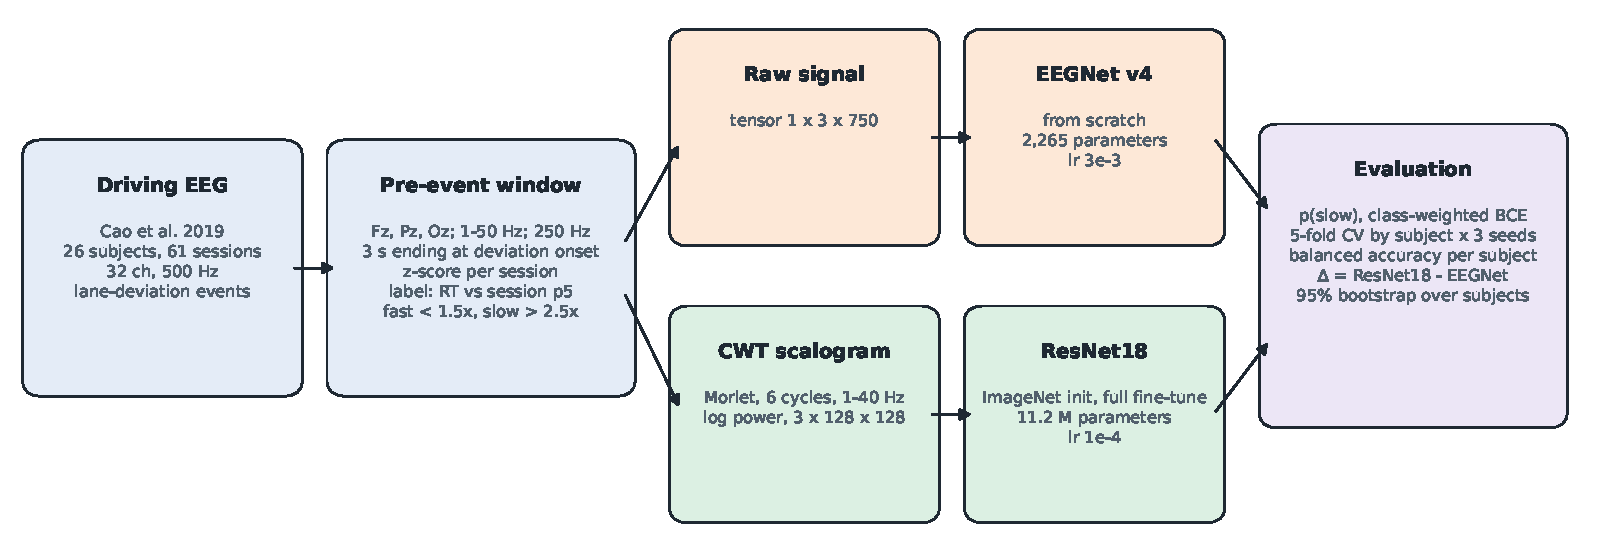
\includegraphics[width=0.95\textwidth]{pipeline}
\caption{Pipeline. The same pre-event windows, labels, folds and seeds feed both branches; only the representation and the network differ. Evaluation is always on subjects held out from training and early stopping.}
\label{fig:pipeline}
\end{figure*}

Fig.~\ref{fig:pipeline} summarizes the pipeline, and Fig.~\ref{fig:repr} shows the three representations of one fast and one slow window from the same session.

\begin{figure*}[t]
\centering
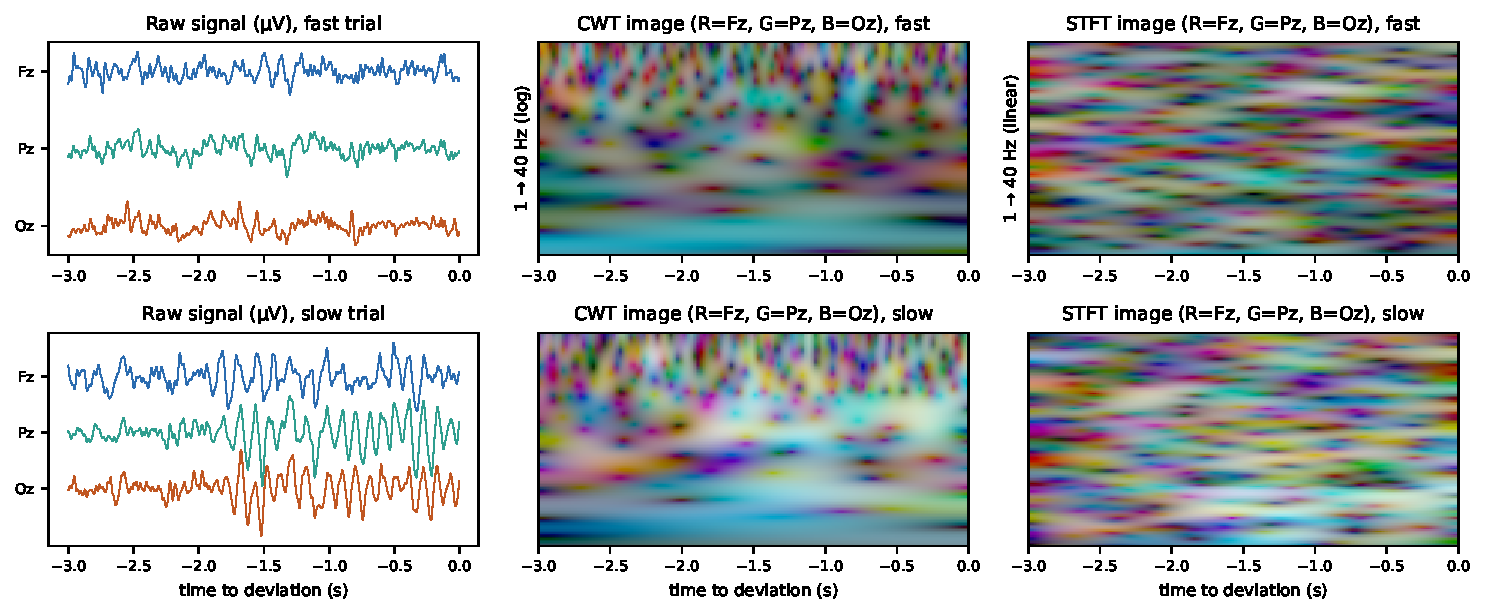
\includegraphics[width=0.92\textwidth]{fig_representaciones}
\caption{One fast and one slow window from the same session in the three representations. Images show session z-scored log power, with Fz, Pz and Oz as the R, G and B channels. The slow window shows posterior alpha bursts (Pz, Oz) that appear in both images as bright bands in the 8--13\,Hz range.}
\label{fig:repr}
\end{figure*}

\subsection{Data representation}
\textbf{Raw signal.} The continuous recording is band-passed (zero-phase Butterworth, order 4, 1--50\,Hz) before windowing and decimated from 500 to 250\,Hz. Each window is z-scored per session and channel.

\textbf{Scalogram (main).} Continuous wavelet transform with a complex Morlet wavelet (6 cycles), 128 log-spaced frequencies from 1 to 40\,Hz, with reflected edges~\cite{torrence1998}. Log power is z-scored per session, channel and frequency, clipped at $\pm3$, resized to 128 time bins, and stored as 8-bit values. Fz, Pz and Oz become the R, G and B channels.

\textbf{Spectrogram (ablation).} Short-time Fourier transform with a 1\,s Hann window and 24\,ms hop, 1--40\,Hz on a linear axis, resized to $128\times128$, with the same scaling.

\subsection{Architectures}
\textbf{EEGNet v4}~\cite{lawhern2018} (baseline): temporal convolution ($F_1=8$, kernel 125 = 0.5\,s), depthwise spatial convolution ($D=2$) with max-norm 1, separable convolution ($F_2=16$, kernel 32), average pooling, dropout 0.5, and a linear head with max-norm 0.25. Input $1\times3\times750$, one logit, \textbf{2{,}265 parameters}, trained from scratch.

\textbf{ResNet18}~\cite{he2016} (main): ImageNet weights~\cite{deng2009}, all layers fine-tuned, final layer replaced by a 512$\to$1 linear head. Input $3\times128\times128$ normalized with ImageNet statistics, \textbf{11{,}177{,}025 parameters}. The pretrained weights only initialize generic visual filters; that they transfer to scalograms is an assumption that the no-pretraining ablation tests.

\begin{table}[t]
\centering
\caption{Tensor shapes (batch omitted) and parameter counts.}
\label{tab:arch}
\footnotesize
\begin{tabular}{@{}llr@{}}
\toprule
Layer & Output shape & Params \\
\midrule
\multicolumn{3}{@{}l}{\emph{EEGNet v4 (raw signal)}} \\
Input & $1\times3\times750$ & -- \\
Temporal conv $1\times125$, 8 filters + BN & $8\times3\times750$ & 1{,}016 \\
Depthwise spatial conv $3\times1$, $D{=}2$ & $16\times1\times750$ & 48 \\
BN, ELU, avg-pool $1\times4$, dropout & $16\times1\times187$ & 32 \\
Separable conv $1\times32$ + $1\times1$, BN & $16\times1\times187$ & 800 \\
ELU, avg-pool $1\times8$, dropout, flatten & $368$ & -- \\
Linear $\to$ logit & $1$ & 369 \\
\emph{Total} & & \emph{2{,}265} \\
\midrule
\multicolumn{3}{@{}l}{\emph{ResNet18 (scalogram)}} \\
Input (ImageNet-normalized) & $3\times128\times128$ & -- \\
Conv $7\times7$/2, BN, ReLU, max-pool/2 & $64\times32\times32$ & 9{,}536 \\
Stage 1 (2 basic blocks) & $64\times32\times32$ & 147{,}968 \\
Stage 2 (2 basic blocks, /2) & $128\times16\times16$ & 525{,}568 \\
Stage 3 (2 basic blocks, /2) & $256\times8\times8$ & 2{,}099{,}712 \\
Stage 4 (2 basic blocks, /2) & $512\times4\times4$ & 8{,}393{,}728 \\
Global avg-pool, linear $\to$ logit & $1$ & 513 \\
\emph{Total} & & \emph{11{,}177{,}025} \\
\bottomrule
\end{tabular}
\end{table}

\subsection{Objective and optimization}
Both models minimize class-weighted binary cross-entropy on the slow-class logit $z$:
\begin{equation}
\mathcal{L} = -\tfrac{1}{N}\textstyle\sum_i \big[w\,y_i\log\sigma(z_i) + (1-y_i)\log(1-\sigma(z_i))\big],
\end{equation}
with $w=N_{\text{fast}}/N_{\text{slow}}$ computed on the training subjects. Optimizer: AdamW~\cite{loshchilov2019}, weight decay 0.01, constant learning rate, batch 128 (EEGNet) or 64 (ResNet18), at most 80 epochs, early stopping with patience 8 on the AUROC of 4 training subjects held out as internal validation (the same subjects for every model). The decision threshold is 0.5. There is no data augmentation.

\textbf{Matched tuning.} Each model received the same search: three learning rates on seed 0, selected only by internal-validation AUROC. EEGNet: $\{3\!\times\!10^{-4}, 10^{-3}, 3\!\times\!10^{-3}\}$, selected $3\!\times\!10^{-3}$ (AUROC 0.883). ResNet18: $\{10^{-5}, 3\!\times\!10^{-5}, 10^{-4}\}$, selected $10^{-4}$ (AUROC 0.868).

\begin{table}[t]
\centering
\caption{Learning-rate search (seed 0, 5 folds): internal-validation AUROC and median best epoch. Test folds are not used.}
\label{tab:lr}
\footnotesize
\begin{tabular}{@{}lccc@{}}
\toprule
Model & lr & Val.\ AUROC & Best epoch \\
\midrule
EEGNet & $3\times10^{-4}$ & 0.863 & 12 \\
EEGNet & $10^{-3}$ & 0.870 & 11 \\
EEGNet & $\mathbf{3\times10^{-3}}$ & \textbf{0.883} & 14 \\
ResNet18 & $10^{-5}$ & 0.825 & 3 \\
ResNet18 & $3\times10^{-5}$ & 0.844 & 1 \\
ResNet18 & $\mathbf{10^{-4}}$ & \textbf{0.868} & 1 \\
\bottomrule
\end{tabular}
\end{table}

\section{Experimental protocol}
\textbf{Dataset.} Cao et al.~\cite{cao2019,cao2019figshare}: 27 subjects, 62 sessions of simulated driving with lane deviations, 32-channel EEG at 500\,Hz (figshare v2, CC BY 4.0). Session \texttt{s04\_051130m} was dropped as a duplicate of \texttt{s05\_051120m}: all 32 EEG channels and all 1{,}083 events are sample-identical, and only the vehicle-position channel differs. This leaves 26 subjects and 61 sessions. Session names end in \emph{m} (motion platform) or \emph{n} (motionless).

\textbf{Exclusions.} RT $<0.1$\,s (likely marker errors) or $>60$\,s; windows overlapping the previous response (7.0\% of trials); and windows with peak amplitude above 150\,\textmu V (0.67\%), which were mostly fast and would give a noise shortcut. The final set has \textbf{18{,}087 windows}: 13{,}094 fast and 4{,}993 slow (27.6\%). Table~\ref{tab:data} gives the flow. Subjects contribute between 127 and 1{,}843 windows; subjects 14 and 55 have almost no slow windows (2 and 0), which is why 24 of 26 subjects enter the per-subject metric.

\begin{table}[t]
\centering
\caption{Data flow from trials to windows.}
\label{tab:data}
\footnotesize
\begin{tabular}{@{}lr@{}}
\toprule
Step & Count \\
\midrule
Lane-deviation trials, 61 sessions & 27{,}171 \\
\quad excluded: RT $<0.1$\,s & 2.5\% \\
\quad excluded: RT $>60$\,s & 67 \\
\quad excluded: window overlaps previous response & 7.0\% \\
\quad discarded: intermediate RT ($1.5$--$2.5\,r_s$) & -- \\
Clearly fast or slow windows & 18{,}209 \\
\quad excluded: peak amplitude $>150$\,\textmu V & 122 \\
\textbf{Final windows} (fast / slow) & \textbf{18{,}087} (13{,}094 / 4{,}993) \\
Subjects / sessions / folds & 26 / 61 / 5 \\
\bottomrule
\end{tabular}
\end{table}

\textbf{Split.} 5-fold cross-validation by subject: all sessions of a subject are in the same fold, and the folds are balanced by window count (about 3{,}600 per fold) and stored in \texttt{folds.csv}. Every model uses the same folds and seeds 0, 1, 2, giving 15 trainings per model. The test fold never takes part in training, early stopping, or learning-rate selection.

\textbf{Baselines and controls.} (i) EEGNet on the raw signal (neural baseline). (ii) Logistic regression on log band power (theta, alpha, beta; 9 features), with and without session z-scoring (classical baseline). (iii) Logistic regression on the trial's relative position in the session (time-on-task drift control). (iv) The band-power model trained on labels shuffled within session (chance control).

\textbf{Metrics.} Primary: per-subject balanced accuracy (BA). Secondary: AUROC. Diagnostic: number of subjects above 0.5, per-condition BA, and the channel/band EEGNet variants. Qualitative: class-mean scalograms and Grad-CAM~\cite{selvaraju2017}. Table~\ref{tab:metrics} states what each does not establish.

\textbf{Chance level.} Besides the retrained shuffled-label control, we run a permutation test on the stored test predictions of each network~\cite{ojala2010} (2{,}000 permutations) under two nulls: labels shuffled within session, and labels circularly shifted within session, which preserves the temporal clustering of slow trials. This tests predictions, not retrained models.

\textbf{Compute and reproducibility.} The main comparison and all ablations ran on one Apple M1 Pro (PyTorch 2.10, MPS backend, float32). A replication of the main ResNet18 ran on an NVIDIA RTX 3080 (CUDA, mixed precision). Time per ResNet18 epoch is about 23\,s on MPS and 11\,s on CUDA. Every setting is in \texttt{config.yaml}; \texttt{python train.py all} and \texttt{python evaluate.py} reproduce all tables and figures. Checkpoints and the 0.8\,GB image arrays are regenerated rather than versioned.

\begin{table}[t]
\centering
\caption{Metrics and what they do not establish.}
\label{tab:metrics}
\footnotesize
\begin{tabular}{@{}p{0.27\columnwidth}p{0.63\columnwidth}@{}}
\toprule
Metric & Does \emph{not} establish \\
\midrule
Per-subject BA (primary) & That the model detects drowsiness physiologically (classes are RT-defined), or that it transfers to other tasks or to the same person over time. \\
AUROC & That probabilities are calibrated, or performance at a given threshold. \\
Subjects above 0.5 & A mechanism; it only shows the spread between people. \\
Permutation test & Chance for a \emph{retrained} model; predictions are kept fixed. \\
Scalograms, Grad-CAM & That highlighted regions are causal; this is interpretation. \\
\bottomrule
\end{tabular}
\end{table}

\section{Results}
\begin{table*}[t]
\centering
\caption{Performance on unseen subjects. BA and AUROC: mean $\pm$ SD over 15 runs (5 folds $\times$ 3 seeds). Per-subject BA: mean over 24 subjects (seeds averaged), with 95\% subject-bootstrap CI. Main comparison in bold.}
\label{tab:main}
\small
\begin{tabular}{@{}llcccc@{}}
\toprule
Model & Input & BA & AUROC & Per-subject BA [95\% CI] & Subj.\ $>0.5$ \\
\midrule
Shuffled labels (chance control) & band power & 0.495 $\pm$ 0.008 & 0.491 & 0.491 [0.482, 0.501] & 8 of 24 \\
Trial position (drift control) & trial index & 0.554 $\pm$ 0.025 & 0.584 & 0.567 [0.536, 0.595] & 20 of 24 \\
\midrule
Band power + LR, session z-score & band power & 0.683 $\pm$ 0.049 & 0.740 & 0.706 [0.677, 0.738] & 24 of 24 \\
Band power + LR & band power & 0.718 $\pm$ 0.052 & 0.783 & 0.681 [0.654, 0.709] & 24 of 24 \\
\midrule
ResNet18, CWT, no pretraining & CWT image & 0.742 $\pm$ 0.051 & 0.825 & 0.735 [0.715, 0.757] & 24 of 24 \\
ResNet18, STFT, ImageNet & STFT image & 0.753 $\pm$ 0.046 & 0.826 & 0.751 [0.728, 0.774] & 24 of 24 \\
\midrule
ResNet18, CWT, ImageNet (CUDA replication) & CWT image & 0.759 $\pm$ 0.044 & 0.837 & 0.754 [0.732, 0.776] & 24 of 24 \\
EEGNet, lr 1e-3, 40 epochs (initial run) & raw $3\times750$ & 0.779 $\pm$ 0.051 & 0.846 & 0.766 [0.744, 0.788] & 24 of 24 \\
\midrule
\textbf{ResNet18, CWT, ImageNet (main)} & \textbf{CWT image} & \textbf{0.753 $\pm$ 0.048} & \textbf{0.832} & \textbf{0.750 [0.727, 0.773]} & \textbf{24 of 24} \\
\textbf{EEGNet, raw signal (main baseline)} & \textbf{raw $3\times750$} & \textbf{0.788 $\pm$ 0.045} & \textbf{0.855} & \textbf{0.774 [0.753, 0.795]} & \textbf{24 of 24} \\
\bottomrule
\end{tabular}

\end{table*}

\begin{figure*}[t]
\centering
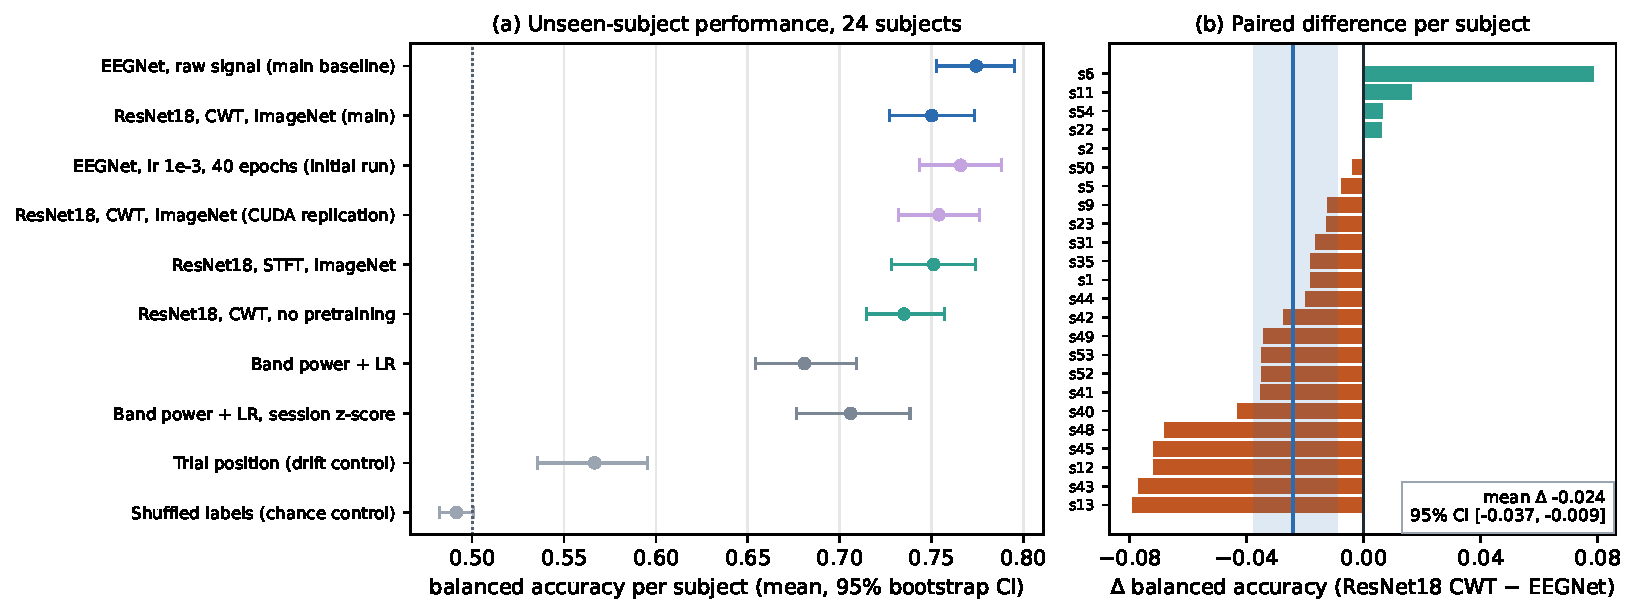
\includegraphics[width=0.92\textwidth]{fig_resultados}
\caption{(a) Per-subject balanced accuracy with 95\% subject-bootstrap CI. (b) Paired difference per subject for the main comparison. Orange: EEGNet better; green: ResNet18 better. The shaded band is the 95\% CI of the mean.}
\label{fig:results}
\end{figure*}

\textbf{Main comparison.} Table~\ref{tab:main} and Fig.~\ref{fig:results} show the result. EEGNet on the raw signal reaches \eegMainSubj{} per-subject BA and ResNet18 on scalograms \resMainSubj{}. The paired difference is $\Delta=\deltaMain$ with 95\% CI \ciMain{}; ResNet18 is better in \resBetter{} subjects. \textbf{Under the pre-registered rule, the hypothesis is not supported}: \mainVerdict{}

\textbf{Robustness of the conclusion.} The conclusion does not depend on the run. Against the initial EEGNet configuration (lr $10^{-3}$, 40-epoch cap), $\Delta=\deltaInitial$; using the CUDA replication of ResNet18 instead, $\Delta=\deltaCuda$. The CUDA and MPS ResNet18 runs differ by $\deltaCudaMps$ (CI \ciCudaMps), within hardware-level nondeterminism.

\textbf{Against baselines and chance.} Both networks beat the classical band-power models (0.681 and 0.706 per subject, without and with session z-scoring) and the trial-position control (0.567), so time on task alone explains little. The shuffled-label control gives 0.491. In the permutation test on stored predictions, the per-subject chance level is about 0.51--0.52 under both nulls, including the conservative circular-shift null. Every network's observed BA exceeds all 2{,}000 permutations ($p<0.001$).

\begin{table}[t]
\centering
\caption{Permutation test on stored test predictions (2{,}000 permutations, per-subject BA). The circular-shift null preserves the temporal clustering of slow trials.}
\label{tab:perm}
\footnotesize
\begin{tabular}{@{}lcccc@{}}
\toprule
Model & Observed & Shuffle & Shift & $p$ \\
\midrule
EEGNet (main) & 0.774 & 0.517 & 0.516 & $<$0.001 \\
ResNet18 CWT (main) & 0.761 & 0.512 & 0.511 & $<$0.001 \\
ResNet18 STFT & 0.755 & 0.511 & 0.510 & $<$0.001 \\
ResNet18 CWT, $10^{-4}$ & 0.750 & 0.512 & 0.511 & $<$0.001 \\
ResNet18 STFT, $10^{-4}$ & 0.751 & 0.512 & 0.511 & $<$0.001 \\
ResNet18 scratch & 0.735 & 0.509 & 0.508 & $<$0.001 \\
ResNet18 CWT, $10^{-4}$, CUDA & 0.754 & 0.513 & 0.512 & $<$0.001 \\
EEGNet (initial) & 0.766 & 0.518 & 0.517 & $<$0.001 \\
\bottomrule
\end{tabular}

\end{table}

\textbf{Uncertainty.} The standard deviation across fold--seed runs (about 0.05) is dominated by which subjects fall in the test fold, not by seed. This is why inference is done on paired per-subject differences.

\section{Ablations and controlled comparisons}
Each comparison changes one factor and is paired by subject (Table~\ref{tab:main}, ablation rows).

\textbf{Pretraining (initialization).} The same ResNet18 trained from scratch on scalograms reaches \scratchSubj{}. Pretrained minus scratch is $\deltaScratch$, CI \ciScratch{}, so ImageNet initialization helps even though natural images and scalograms differ. The best validation epoch was 1 or 2 in 13 of 15 scratch runs and 1 in 11 of 15 pretrained runs: the 11M-parameter network fits the roughly 14k training windows almost immediately, while EEGNet's median best epoch is 29.

\textbf{Representation (CWT vs.\ STFT).} With everything else fixed (model, initialization, learning rate, folds, seeds, image size, 1--40\,Hz), the STFT spectrogram reaches \stftSubj{}. CWT minus STFT is $\deltaStft$, CI \ciStft{}: \stftSentence{}

\textbf{Which signal carries the information (EEGNet diagnostic).} We retrained EEGNet with a single channel or a band-limited signal (Fig.~\ref{fig:diag}; these variants use the initial EEGNet configuration and are compared with it). Every restriction hurts. Fz alone is the best single channel (0.724 vs.\ 0.766), and removing delta from Fz drops it to 0.635. Delta alone (1--4\,Hz) keeps 0.710, and theta+alpha (4--13\,Hz) gives 0.730. Information is therefore spread across bands, but a large share is low-frequency activity at Fz.

\begin{figure}[t]
\centering
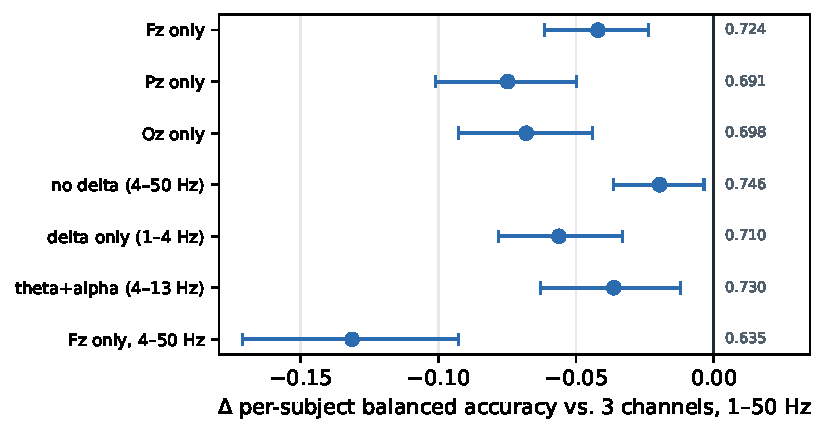
\includegraphics[width=\columnwidth]{fig_diagnostico}
\caption{EEGNet channel and band diagnostic: paired per-subject difference from the 3-channel, 1--50\,Hz model (95\% CI); numbers are the per-subject mean BA. Band limiting is applied to the 3\,s window and leaves edge transients.}
\label{fig:diag}
\end{figure}

\begin{figure*}[t]
\centering
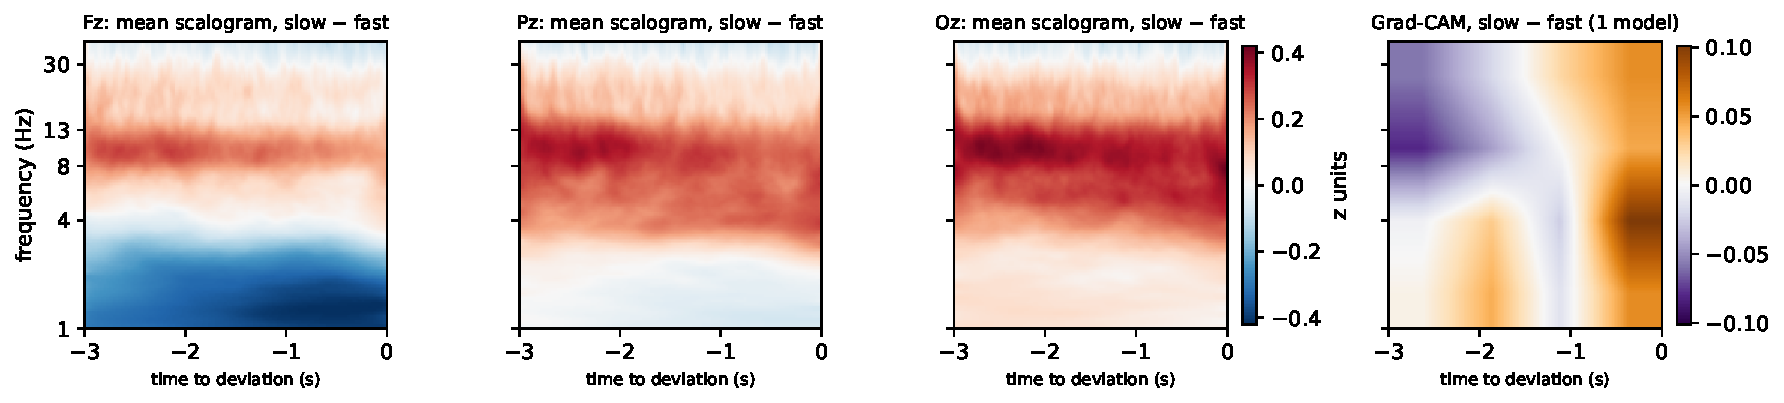
\includegraphics[width=0.95\textwidth]{fig_interpretacion}
\caption{Left three panels: class-mean CWT scalogram per channel over all windows, slow minus fast (session z units). Right: Grad-CAM of one ResNet18 (fold 0, seed 0), slow minus fast, averaged over correctly classified test windows. Grad-CAM is interpretation, not evidence.}
\label{fig:interp}
\end{figure*}

\textbf{Qualitative.} Across all 18{,}087 windows, slow windows have more 4--13\,Hz power over the whole 3\,s at all three channels, strongest at Pz and Oz, and less power below 4\,Hz at Fz (Fig.~\ref{fig:interp}). Because the difference is constant over the window, it looks like a state rather than an event-locked response. This is consistent with theta/alpha changes reported with declining alertness~\cite{jung1997}. Grad-CAM for one network weights 2--8\,Hz near the end of the window for the slow class; we treat this as interpretation, not evidence.

\section{Failure analysis and limitations}
\textbf{Where the models fail.} Per-subject BA ranges from \worstRange{}. The weakest subjects for EEGNet are \worstSubjects{}. They fail in two opposite ways that both point to a learned base rate. Subjects with few slow trials (9 and 6) are classified as fast almost always: the true-positive rate for slow is 0.42--0.43, while the true-negative rate is 0.97--1.00. Subject 22, the only one with a majority of slow trials, shows the reverse, with a true-negative rate of 0.56. ResNet18 loses most against EEGNet in subjects 13, 43, 45, 12 and 48 ($\Delta$ between $-0.07$ and $-0.08$). The two models agree on \agreePct{} of windows. When they disagree, EEGNet is right more often (\disagree{}). Windows misclassified by both are enriched in slow trials (\bothWrongSlow{} slow vs.\ 27.6\% base rate): missing slow responses is the dominant failure. By condition, BA is \condText{} (Table~\ref{tab:cond}). The motion platform does not change the ranking of the models.

\begin{table}[t]
\centering
\caption{Balanced accuracy by session condition (pooled windows of each condition, mean over seeds). Descriptive only.}
\label{tab:cond}
\footnotesize
\begin{tabular}{@{}lcc@{}}
\toprule
Model & Motion (m) & Motionless (n) \\
\midrule
EEGNet (initial) & 0.780 & 0.773 \\
EEGNet (main) & 0.791 & 0.782 \\
ResNet18 CWT (CUDA) & 0.758 & 0.762 \\
ResNet18 CWT (main) & 0.752 & 0.748 \\
ResNet18 scratch & 0.743 & 0.744 \\
ResNet18 STFT & 0.743 & 0.758 \\
\midrule
Sessions / windows & 27 / 6{,}907 & 34 / 11{,}180 \\
Slow proportion & 0.328 & 0.244 \\
\bottomrule
\end{tabular}

\end{table}

\begin{figure}[t]
\centering
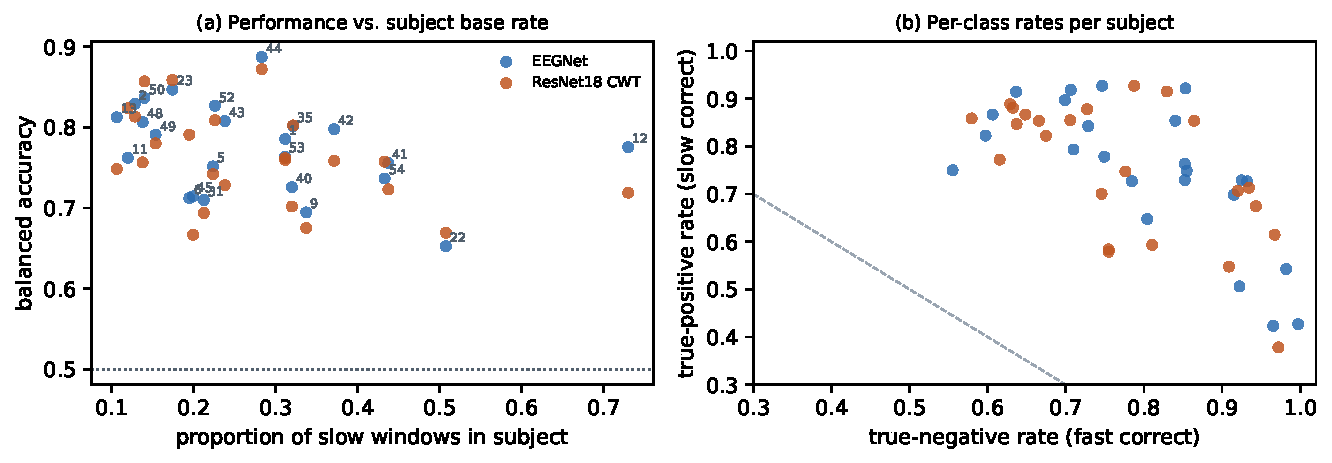
\includegraphics[width=\columnwidth]{fig_fallos}
\caption{Failure analysis per subject (24 subjects). (a) Balanced accuracy against each subject's proportion of slow windows. (b) True-positive (slow) against true-negative (fast) rate; the dashed line is chance. Subjects in the lower right miss most slow responses.}
\label{fig:fallos}
\end{figure}

Fig.~\ref{fig:fallos}(b) shows the asymmetry directly: most low-performing points lie in the lower right, with high specificity and low sensitivity for slow responses. Because slow labels are session-relative, a subject whose slow trials are rare and only moderately slow offers little contrast, and a model trained on other people sets its threshold for the population's base rate rather than the subject's.

\textbf{Possible non-neural signal.} The low-frequency difference at Fz could reflect eye movements or blinks rather than cortical activity, and the 150\,\textmu V rule removes only large artifacts. That Fz delta carries much of the information makes this the main threat to a neural interpretation, and it is the first thing to check (e.g., with ICA or EOG regression) before transferring the result to pain or trust.

\textbf{Other limitations.} (1) Labels are behavioral and session-relative, not a ground truth of drowsiness. (2) Per-session normalization uses unlabeled test-session data. (3) Slow trials cluster in time (the probability that a trial is slow is 0.65 after a slow trial and 0.13 after a fast one), so windows are not independent; we only resample subjects. (4) EEGNet's best epoch was 79 of 80 in one run and above 60 in two more, so the baseline may be slightly under-trained; more epochs could only widen the gap against the hypothesis. (5) ResNet18 peaks within 1--3 epochs, so its effective tuning budget is small. A lower learning rate did not help on validation, but schedules, augmentation, or freezing layers were not explored. (6) Results hold for this dataset, task, and three channels. We do not extend them to trust or pain without our own data; any such extension is speculation.

\section{Discussion: observation, interpretation, speculation}
\textbf{Observed.} The ordering is the same in every paired comparison we ran. EEGNet on the raw signal is first, followed by the pretrained ResNet18 on CWT, the ResNet18 trained from scratch, the classical band-power models, and the controls. The paired difference between the two main models is small in absolute terms (about 2 points of balanced accuracy), but it is consistent across subjects (EEGNet better in \eegBetter{} of 24) and across hardware.

\textbf{Interpreted.} Three facts together suggest why images do not help. First, the class difference is a sustained spectral shift (Fig.~\ref{fig:interp}), which a temporal convolution with a 0.5\,s kernel followed by pooling can capture directly; the image adds no information that the raw signal lacks, since the scalogram is a fixed transform of it. Second, the ResNet18 reaches its best validation AUROC within one or two epochs. Its capacity is far larger than the roughly 14k training windows warrant, and early stopping effectively turns it into a lightly adapted ImageNet feature extractor. Third, pretraining helps that extractor, so the CNN benefits from generic low-level filters, but not enough to overcome its mismatch with the input. These are plausible explanations, not tested mechanisms: we did not run, for instance, a ResNet18 on the raw signal or an EEGNet on images.

\textbf{Speculative.} If the same pattern held in pain or trust data, compact raw-signal models would be the better starting point for small, highly variable cohorts. This is untested and is exactly what the next thesis steps will check.

\section{Conclusion}
\textbf{Observation.} On unseen subjects, under matched data, folds, seeds, objective, early stopping, and learning-rate search, a 2k-parameter EEGNet on the raw signal is at least as good as an 11M-parameter ImageNet ResNet18 on wavelet scalograms, and the pre-registered hypothesis is not supported. ImageNet pretraining helps the CNN, and the choice of wavelet over STFT \stftShort{}. \textbf{Interpretation.} Converting EEG to images adds parameters and a transfer assumption without adding information the raw-signal network cannot extract, at least for three channels and 3\,s windows. \textbf{Speculation (untested).} The same may hold for pain and trust decoding.

\textbf{Next thesis steps.} Juan Pablo will apply the pipeline to his CARLA trust dataset once it reaches 40 subjects. Alberto will apply the same protocol (subject-wise cross-validation, per-session calibration, raw-signal EEGNet vs.\ scalogram ResNet18, subject bootstrap) to predict subject-relative pain intensity once his pain dataset reaches 40 subjects. Given this result, he will start from EEGNet on the raw signal and repeat the channel/band diagnostic to rule out ocular and muscle artifacts, a larger risk in pain paradigms than in driving.

\bibliographystyle{IEEEtran}
\bibliography{refs}

\appendix
\section*{Appendix: reproduction}
Code, configuration, results, and figures are in the project repository. \texttt{python train.py prepare} builds windows, folds, baselines, and images from the dataset. \texttt{python train.py all} runs every training. \texttt{python evaluate.py} produces the summary, learning-rate selection, permutation test, paired bootstrap, and per-subject analysis. \texttt{python src/figuras\_reporte.py} regenerates the figures and table in this report. All resampling uses fixed seeds.

\end{document}
